\documentclass[a4paper,11pt,abstracton,hidelinks]{scrartcl}
\usepackage{dphil}
\usepackage{wasysym}
\addbibresource{refs.bib}
% hide section numbers
\setcounter{secnumdepth}{0}


\title{
Chapter 4. Population structure and genetic diversity
}


\author{}


\begin{document}
\renewcommand{\abstractname}{Summary}


\maketitle


%%%%%%%%%%%%%%%%%%%%%%%%%%%%%%%%%%%%%%%%%%%%%%%%%%%%%%%%%%%%%%%%%%%%%%%%%%%%%%%
%%%%%%%%%%%%%%%%%%%%%%%%%%%%%%%%%%%%%%%%%%%%%%%%%%%%%%%%%%%%%%%%%%%%%%%%%%%%%%%
%%%%%%%%%%%%%%%%%%%%%%%%%%%%%%%%%%%%%%%%%%%%%%%%%%%%%%%%%%%%%%%%%%%%%%%%%%%%%%%
\begin{abstract}


@@


\end{abstract}


\tableofcontents


%%%%%%%%%%%%%%%%%%%%%%%%%%%%%%%%%%%%%%%%%%%%%%%%%%%%%%%%%%%%%%%%%%%%%%%%%%%%%%%
%%%%%%%%%%%%%%%%%%%%%%%%%%%%%%%%%%%%%%%%%%%%%%%%%%%%%%%%%%%%%%%%%%%%%%%%%%%%%%%
%%%%%%%%%%%%%%%%%%%%%%%%%%%%%%%%%%%%%%%%%%%%%%%%%%%%%%%%%%%%%%%%%%%%%%%%%%%%%%%
\section{Introduction}\label{sec:introduction}


%
In the previous chapter I described the \textit{Anopheles gambiae} 1000 Genomes Project (Ag1000G) phase 1 data resource, which comprises genome variation data from 765 individual mosquitoes sampled from 8 countries spanning sub-Saharan Africa, and includes representation of both \textit{An. gambiae} and \textit{An. coluzzii}.
%
The availability of genomic data from multiple species and geographical locations provides an opportunity to investigate many facets of their population biology and demography.
%
In this chapter I describe analyses of the Ag1000G phase 1 data investigating genetic population structure among the mosquito populations sampled, and characterising levels of genetic diversity within and differentiation between populations.
%
These analyses are interesting because they allow us to begin to build a picture of the underlying demography of these populations, including variations in population size over time and space, and in the degree of connectivity between populations.
%
Exploring these heterogeneities is particularly relevant because \textit{An. gambiae} and \textit{An. coluzzii} both have an extremely broad geographical and ecological range~\citep{Wiebe2017}.
%
\textit{An. coluzzii} is found from the West Coast throughout West and Central Africa.
%
The range of \textit{An. gambiae} overlaps that of \textit{An. coluzzii} and extends across the Great Rift to the East coast, stretching down to South Africa.
%
Both species' ranges span the equator and encompass a remarkably diverse range of environments, including coastal, savanna, sahel and rainforest @@cite.
%
Human population density and land use, and the history and current coverage of malaria vector control interventions, also vary substantially throughout this range @cite.
%
While we do not have the sampling resolution to attempt to correlate any of these individual variables with genetic features of mosquito populations, we can begin to highlight major variations between populations and generate hypotheses for further investigation.
%


@@todo something about collaboration with others


%%%%%%%%%%%%%%%%%%%%%%%%%%%%%%%%%%%%%%%%%%%%%%%%%%%%%%%%%%%%%%%%%%%%%%%%%%%%%%%
%%%%%%%%%%%%%%%%%%%%%%%%%%%%%%%%%%%%%%%%%%%%%%%%%%%%%%%%%%%%%%%%%%%%%%%%%%%%%%%
%%%%%%%%%%%%%%%%%%%%%%%%%%%%%%%%%%%%%%%%%%%%%%%%%%%%%%%%%%%%%%%%%%%%%%%%%%%%%%%
\section{Results}\label{sec:results}


%%%%%%%%%%%%%%%%%%%%%%%%%%%%%%%%%%%%%%%%%%%%%%%%%%%%%%%%%%%%%%%%%%%%%%%%%%%%%%%
%%%%%%%%%%%%%%%%%%%%%%%%%%%%%%%%%%%%%%%%%%%%%%%%%%%%%%%%%%%%%%%%%%%%%%%%%%%%%%%
\subsection{The influence of genome architecture on population structure}\label{subsec:treescan}


My goal in this chapter is to investigate genetic population structure, which means studying the extent to which individual mosquitoes are genetically related to each other, and identifying groups of individuals which are more or less related.
%
The Ag1000G phase 1 resource comprises data on more than 52 million single nucleotide polymorphisms (SNPs) distributed throughout the genome, and thus provides an extremely rich and high-resolution source of information with which to investigate population structure.
%
However, a complication arises because previous genomic studies of \textit{An. gambiae} and \textit{An. coluzzii} have shown that different regions of the genome can convey both quantitatively and qualitatively  different information about how individuals are related to each other.
%
In particular, several studies have found that differentiation between the two species \textit{An. gambiae} and \textit{An. coluzzii} is particularly high within certain genome regions but lower or almost absent elsewhere @@cite.
%
There are also a number of large chromosomal inversions that are polymorphic within one or both of these species @@cite.
%
Chromosomal inversions cause a greatly reduced rate of recombination between different karyotypes @@cite, which in turn will affect patterns of relatedness between individuals.
%
Any analysis of population structure that fails to take these heterogeneities into account will struggle to present a clear picture.
%


\begin{figure}[t!]
\centering
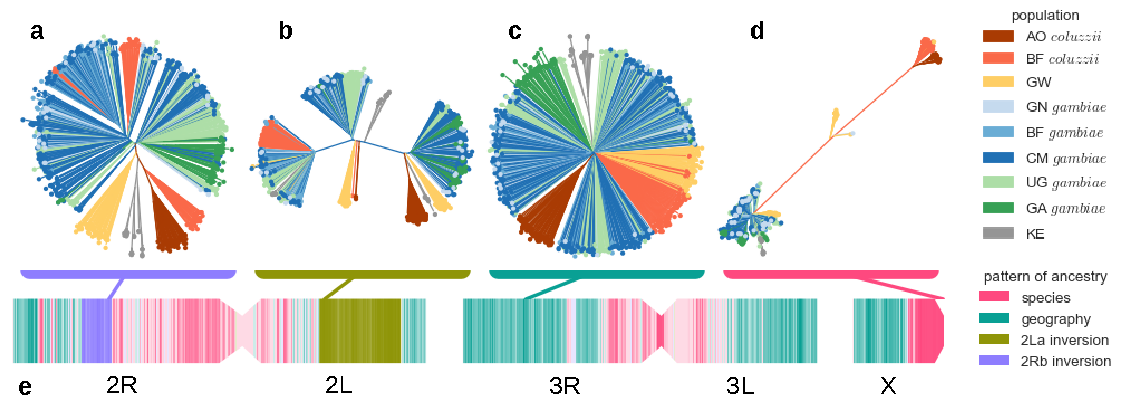
\includegraphics[width=\textwidth]{artwork/chapter4/treescan.pdf}
\caption{Variation across the genome in patterns of relatedness between individual mosquitoes.
%
Panels \textbf{a-d} each show a neighbour-joining tree computed from pairwise genetic distances within a specific 200 kb genomic window, illustrating the four most common patterns of relatedness found throughout the genome.
%
\textbf{a}, Example of tree within the 2Rb inversion.
%
\textbf{b}, Example of tree within the 2La inversion.
%
\textbf{a}, Example of tree from euchromatic region of Chromosome 3.
%
\textbf{a}, Example of tree pericentromeric region of the X chromosome.
%
\textbf{e}, Painting of the genome illustrating where the four major patterns of relatedness are found.
%
Each 200 kb window is painted with a colour to indicate which of the four major patterns of relatedness it is most strongly correlated with.
%
}
\label{fig:treescan}
\end{figure}


To explore the relationship between genetic population structure and genome architecture, I divided the genome into @@ non-overlapping @@ kb windows, and then computed pairwise genetic distance between individuals within each window separately.
%
For each window I computed a neighbour-joining tree and visualised each of the resulting trees as an unrooted dendrogram.
%
Several qualitatively different tree topologies were evident in different genome regions (e.g., Fig.~\ref{fig:treescan}a-d).
%
For example, within the pericentromeric region of the X chromosome, trees showed extremely strong clustering by species (e.g., Fig.~\ref{fig:treescan}d).
%
In contrast, trees from euchromatic regions of Chromosome 3 showed some clustering by geographical location, but no clustering by species at all (e.g., Fig.~\ref{fig:treescan}c).
%
Trees within the 2Rb and 2La inversions also had unique topologies, consistent with clustering by inversion karyotype (e.g., Fig.~\ref{fig:treescan}a,b).
%


To explore these variations in tree topology systematically, I computed the Pearson correlation coefficient between distance matrices from all pairs of genomic windows.
%
I then performed dimensionality reduction on the resulting correlation matrix via multidimensional scaling, to identify common patterns of relatedness found in multiple genome windows.
%
The first three principal coordinates (PCs) from this analysis displayed a strong association with specific patterns of relatedness and genome regions.
%
To visualise these results, I devised a transformation from these first three PCs to different colours representing the different patterns of relatedness, and used these to paint the associated genome windows (Fig.~\ref{fig:treescan}e).
%
The first PC identified the common pattern of relatedness found throughout the 2La inversion.
%
The third PC identified the pattern of relatedness found within the 2Rb inversion.
%
The second PC identified the contrast between the highly species-driven patterns of relatedness found generally in pericentromeric regions particularly of the X chromosome, and the more geographically-driven patterns found in euchromatic regions of X chromosome and Chromosome 3.
%
There were also a minority of genome windows which did not display a strong correlation any of these major patterns of relatedness, shown in Fig~\ref{fig:treescan}e as paler colours.
%
These included the windows spanning the insecticide resistance gene \textit{Vgsc} which is found near to the centromere of chromosome arm 2L, and which is known to have experienced adaptive introgression between \textit{An. gambiae} and \textit{An. coluzzii} @@cite.
%
This provides a clue that windows affected by strong positive selection may display unusual patterns of gene flow between countries and/or species, explored further in Chapter 6.


%%%%%%%%%%%%%%%%%%%%%%%%%%%%%%%%%%%%%%%%%%%%%%%%%%%%%%%%%%%%%%%%%%%%%%%%%%%%%%%
%%%%%%%%%%%%%%%%%%%%%%%%%%%%%%%%%%%%%%%%%%%%%%%%%%%%%%%%%%%%%%%%%%%%%%%%%%%%%%%
%%%%%%%%%%%%%%%%%%%%%%%%%%%%%%%%%%%%%%%%%%%%%%%%%%%%%%%%%%%%%%%%%%%%%%%%%%%%%%%
\section{Methods}\label{sec:methods}


@@


%%%%%%%%%%%%%%%%%%%%%%%%%%%%%%%%%%%%%%%%%%%%%%%%%%%%%%%%%%%%%%%%%%%%%%%%%%%%%%%
%%%%%%%%%%%%%%%%%%%%%%%%%%%%%%%%%%%%%%%%%%%%%%%%%%%%%%%%%%%%%%%%%%%%%%%%%%%%%%%
%%%%%%%%%%%%%%%%%%%%%%%%%%%%%%%%%%%%%%%%%%%%%%%%%%%%%%%%%%%%%%%%%%%%%%%%%%%%%%%
\section{Conclusion}\label{sec:conclusion}


@@


%%%%%%%%%%%%%%%%%%%%%%%%%%%%%%%%%%%%%%%%%%%%%%%%%%%%%%%%%%%%%%%%%%%%%%%%%%%%%%%
%%%%%%%%%%%%%%%%%%%%%%%%%%%%%%%%%%%%%%%%%%%%%%%%%%%%%%%%%%%%%%%%%%%%%%%%%%%%%%%
%%%%%%%%%%%%%%%%%%%%%%%%%%%%%%%%%%%%%%%%%%%%%%%%%%%%%%%%%%%%%%%%%%%%%%%%%%%%%%%
\section{Acknowledgments}\label{sec:acknowledgments}


@@


\printbibliography


\clearpage
\beginsupplement
%%%%%%%%%%%%%%%%%%%%%%%%%%%%%%%%%%%%%%%%%%%%%%%%%%%%%%%%%%%%%%%%%%%%%%%%%%%%%%%
%%%%%%%%%%%%%%%%%%%%%%%%%%%%%%%%%%%%%%%%%%%%%%%%%%%%%%%%%%%%%%%%%%%%%%%%%%%%%%%
%%%%%%%%%%%%%%%%%%%%%%%%%%%%%%%%%%%%%%%%%%%%%%%%%%%%%%%%%%%%%%%%%%%%%%%%%%%%%%%
\section{Supplemental figures}\label{sec:supplemental-figures}


@@


\clearpage
%%%%%%%%%%%%%%%%%%%%%%%%%%%%%%%%%%%%%%%%%%%%%%%%%%%%%%%%%%%%%%%%%%%%%%%%%%%%%%%
%%%%%%%%%%%%%%%%%%%%%%%%%%%%%%%%%%%%%%%%%%%%%%%%%%%%%%%%%%%%%%%%%%%%%%%%%%%%%%%
%%%%%%%%%%%%%%%%%%%%%%%%%%%%%%%%%%%%%%%%%%%%%%%%%%%%%%%%%%%%%%%%%%%%%%%%%%%%%%%
\section{Supplemental tables}\label{sec:supplemental-tables}


@@


\end{document}
